\documentclass[12pt]{report}
\usepackage{graphicx}
\usepackage{hyperref}

\title {
	
\includegraphics[width = .2\linewidth]{University-of-Lugano.png} \break \break
	{\bf\Huge Contextual Inquiry and Analysis}
	\\\large Human-Computer Interaction
	\\\small Academic Year 2017/2018 \break
	\\\large \textbf{Group 7}}
	\author{
	\\\large Alessandra Vicini \\ Edoardo Lunardi \\ Ozren Dabic \\ Pasquale Polverino \\ Paganoni Marco}
\date{March 02, 2018}
\begin{document}
	\pagestyle{empty}
	\maketitle
	\section*{\huge Our Research}
	We started thinking of an application which could organize meetings
	between children based on their interests (hobbies and sports). We
	were aware of the fact that children were our users and, keeping in
	my mind this, we tried to develop an idea, a concept with which
	children could be familiar with: and this was our main "topic" which led the
	interviews with children. The "field visit" let us understand properly
	what children expect from an application: during the interview we ask
	them about our main ideas to put in the app. Indeed we want children
	to be honest and sincere with us, and that is what our inteviwer tried
	to do: our questions were initially about their interest, so that
	we could have been certain of creating something which could meet
	their interests and their passions. We faced also the problem of the
	usage of smartphone: many children have some limitations for example,
	imposed by parents and also by the school which not allow children
	to use their phone on lessons time. Finally we proposed our idea for
	make sure that the application can be used only by children: we
	thought that the access accounts may be given by the school, and also
	children loved this idea. So in general term, our "field visit" has
	asserted our ideas about the app and childre gave us also suggestions,
	which means a lot of us and surely we will try to realize them.\\

	Keeping in mind this type of interview, our type of interview, and we
	red the other of the remaining groups: we noticed that all have asked
	the same type of questions, no more different than ours, but we also
	thought that some were too vague and not specific so that they couldn't
	be used to build the app. Beacuse of this we tried to construct our
	flow model having the goal of designing a sort of profile of all children
	in order to put the most common requests in the app and then tried to
	satisfy everybody.\\

	We organized our work activity affinity diagram grouping the main points
	we have found, reading all the interviews, into bigger subsets, which in the
	end result 9, and then we tried to classify under them all the ideas coming
	from the interviews. The most difficult part was this: found groups under
	which structered our work. Our subsets were thought based on the children
	answers and also we have looked for face the topics argued in class, for
	example the privacy and the safety of the applications, problems whose we
	have also a solution in our app and also children knows it. In the end our diagram
	is composed by three main concepts: what children expects and want from the app,
	how we can deal with this in creating something which attracts them and also ethical
	problems, which must be taken in consideration just because we are talking about
	children. Our work looked this way: \\\\\\
	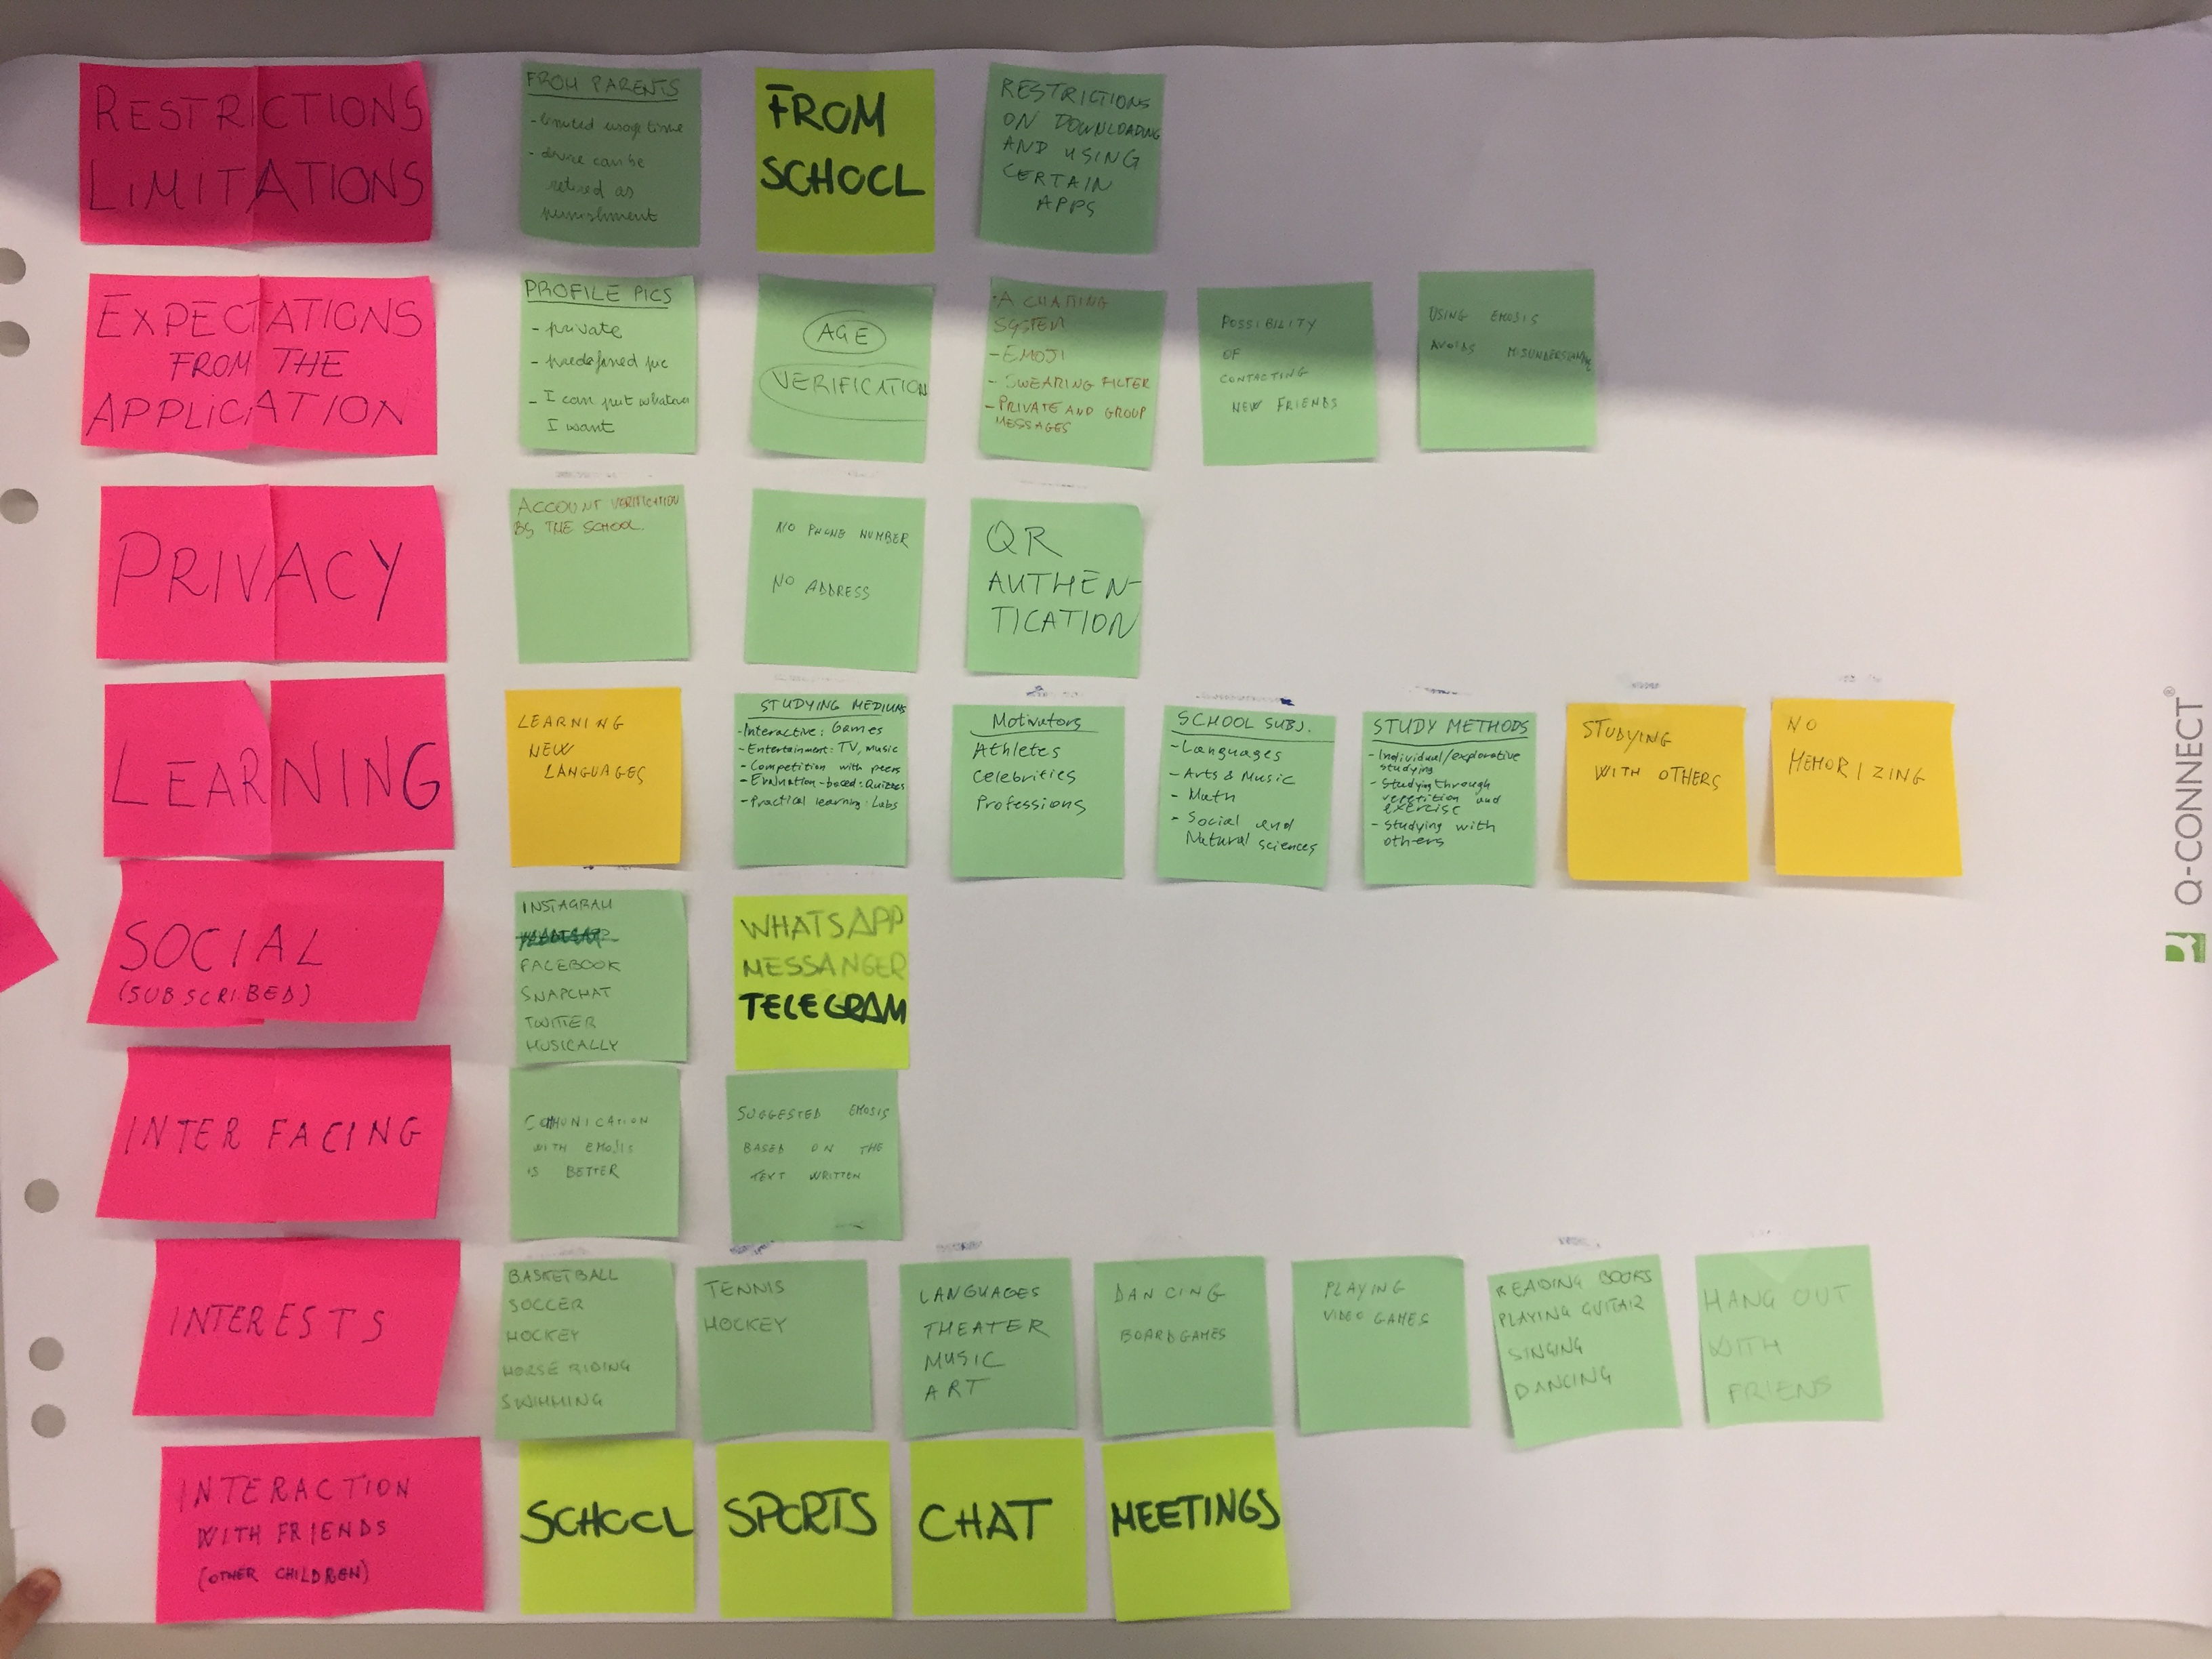
\includegraphics[width = 1.0\linewidth]{affinity_diagram.jpg}\break

  As clearly visible in the diagram we create 9 subsets and each of them has its
  main topics, designed reading the interviews. These are our groups:
	\begin{itemize}
		\item "Restrictions and Limitations":\\
		       we created this subsset because we noticed that the most part of children has
					 restrictions and limitation about the usage of the phone and we tried to face it
					 and not ignored it.
		\item "Expectations from the application" :\\
		       this was an obvious topic to take into consideration, the application is designed
					 for children and they have to be the users: listen to their expectations and request
					 can be just useful. We also noticed that some of their expectations were already part
					 of our idea and these were just confirmed.
		\item "Privacy":\\
		       that is the main problem in the ethical problems and just because our users will be children,
					 we will put more attention on this part and also on how to get the app safe and reliable.
		\item "Learning":\\
		       some children expect an application which help them to learn new things, so even if this wasn't
					 part of our original idea we could think about something like that.
		\item "Social":\\
		       this point focus on the design of the most famous social app: if children are more familiar
					 with a certain type of design, we will try to create something as similar as possible.
		\item "Interfacing":\\
		       many children suggest the usage of emoji in communication: in our app was thought a sort
					 of live chat, so this is a great suggestion for us.
		\item "Interests":\\
		       this is the main topic of our application, so we wrote the most common interests and hobbies
					 so that we can include them in our work.
		\item "Interaction with friends:"\\
		       we make sure that children are used to go out with friends and they have the possibility to do
					 it and if not why not and try to solve the problem.

	\end{itemize}

	 This was our analysis of the project in the entire context, keeping in mind who are our users and what we
	 plan to do considering them. Each part of the project has been structured having in mind children, what we
	 know has been learned by the interview and also analyzing the draws of children. Our group worked toghether
	 to reach the best result possible, we are all satisfied.














	\end {document}
